\section{Periodicity of weighted Catalan numbers}\label{sec:period}
In this section we examine the periodicity of the weighted Catalan numbers modulo a positive integer $m$. In Section~\ref{subsec:period}, we prove the main result which determines if $\{C^b_n\pmod{m}\}$ is periodic. In Section~\ref{subsec:morseperiodicity}, we analyze the specific case of Morse link numbers previously studied by Postnikov and compute periods modulo $7, 11$, and $3^r$. Finally, in Section~\ref{subsec:valuationconjectures} we suggest some conjectures on Morse link numbers to be further explored.

\subsection{Determining when periodicity exists}\label{subsec:period}

We begin with the following lemma on finite continued fractions of the form in Proposition \ref{prop:genfunc}.

\begin{lemma}
\label{lem:cfracexpansion}
For integers $u, v$, let $S_k(u, v)$ denote the set of all sequences $u\leq i_1 < i_2 < \dotsc < i_k\leq v$ of integers such that $i_{m+1}-i_m\geq 2$ for all $m$. For a sequence $b(0), b(1), \dotsc, b(n)$, we have
\[\cfrac{1}{1-\cfrac{b(0)x}{1-\cfrac{b(1)x}{1-\cfrac{b(2)x}{1-\cfrac{\cdots}{1-b(n)x}}}}}=\frac{P(x)}{Q(x)}\]
where $P(x)$ and $Q(x)$ are defined as follows:
\begin{align*}
    P(x) &= 1+\sum_{k\geq 1}\left(\sum_{(i_1, \dotsc, i_k)\in S_k(1, n)}b(i_1)\dotsm b(i_k)\right)(-x)^k \\
    Q(x) &= 1+\sum_{k\geq 1}\left(\sum_{(i_1, \dotsc, i_k)\in S_k(0, n)}b(i_1)\dotsm b(i_k)\right)(-x)^k.
\end{align*}
\end{lemma}
\begin{proof}
    We induct on $n$. For $n=0$ the equality is $\frac{1}{1-b(0)x}=\frac{1}{1-b(0)x}$, which is clearly true. For the inductive step, assume the lemma is true for some $n$. Then
    \[\cfrac{1}{1-\cfrac{b(0)x}{1-\cfrac{b(1)x}{1-\cfrac{b(2)x}{1-\cfrac{\cdots}{1-b(n+1)x}}}}}=\frac{1}{1-b(0)x\frac{P_1(x)}{Q_1(x)}}=\frac{Q_1(x)}{Q_1(x)-b(0)xP_1(x)}\]
    where
    \begin{align*}
    P_1(x) &= 1+\sum_{k\geq 1}\left(\sum_{(i_1, \dotsc, i_k)\in S_k(2, n+1)}b(i_1)\dotsm b(i_k)\right)(-x)^k, \\
    Q_1(x) &= 1+\sum_{k\geq 1}\left(\sum_{(i_1, \dotsc, i_k)\in S_k(1, n+1)}b(i_1)\dotsm b(i_k)\right)(-x)^k
    \end{align*}
    by the inductive hypothesis. Now we have
    \[Q_1(x)-b(0)xP_1(x)=1+\sum_{k\geq 1}\left(\sum_{(i_1, \dotsc, i_k)\in S_k(0, n+1)}b(i_1)\dotsm b(i_k)\right)(-x)^k\]
    because the $P_1(x)$ term accounts for all sequences in $S_k(0, n+1)$ which have $i_1=0$ and the $Q_1(x)$ term accounts for all sequences in $S_k(0, n+1)$ which have $i_1\neq 0$. This proves the inductive step.
\end{proof}

We now have the following key theorem which describes when $C^b_n$ is eventually periodic modulo a positive integer $m$.
\begin{theorem}
\label{thm:periodicity}
Let $m$ be a positive integer. The sequence $\{C^b_n\pmod{m}\}$ is eventually periodic if and only if $m\mid b(0)\dotsm b(k)$ for some positive integer $k$.
\end{theorem}
\begin{proof}
    Using the Dyck path interpretation of Catalan numbers, suppose that $n\mid b(0)\dotsm b(k)$ for some positive integer $k$. Then all paths which exceed height $k$ have a weight that is $0\pmod{m}$, so they can be ignored. This means we may truncate the continued fraction for the weighted Catalan numbers at $b(k)$, so by Lemma \ref{lem:cfracexpansion}, the weighted Catalan numbers have a rational generating function modulo $m$, i.e.
    \[\sum_{n\geq 0}C^b_nx^n\equiv \frac{P(x)}{Q(x)}\pmod{m}\]
    for some polynomials $P, Q$. Furthermore, the constant term of $Q(x)$ is $1$ so this implies a linear recurrence relation $C^b_n\equiv a_1C^b_{n-1}+a_2C^b_{n-2}+\dotsb+a_kC^b_{n-k}\pmod{m}$ for sufficiently large $n$. This proves eventual periodicity because there are only finitely many possibilities for $(C^b_{n-1}, \dotsc, C^b_{n-k})\pmod{m}$, so the sequence eventually repeats.
    
    In the other direction, it suffices to only consider the case where $m=p^r$ for a prime number $p$ and positive integer $r$. We prove the claim by induction on $r$. Suppose that $C^b_n=C^b_{n+k}$ for some period $k$ and sufficiently large integers $n$. Then the generating function of $C^b_n$ is congruent modulo $p^r$ to a function of the form $\frac{P(x)}{Q(x)}$ for polynomials $P, Q$ with constant term $1$, as we may take $Q(x)=1-x^k$ and choose $P$ appropriately. (The choice of $P$ has constant term $1$ because $C^b_0=1$.)
    
    In the base case $r=1$, meaning $m=p$ is a prime, assume for the sake of contradiction that no $b(i)$ is a multiple of $p$. We have
    \[\cfrac{1}{1-\cfrac{b(0)x}{1-\cfrac{b(1)x}{1-\cfrac{b(2)x}{1-\cdots}}}}=\sum_{n\geq0}C_n^bx^n=\frac{P(x)}{Q(x)}=\frac{1+xP_1(x)}{1+xQ_1(x)}\pmod{p}\]
    for some polynomials $P_1, Q_1$ as $P, Q$ both have constant term $1$. By taking the reciprocal, subtracting both sides from $1$, and dividing by $b(0)x$ (recall that we are assuming that $b(0)$ is not a multiple of $p$), we get
    \[\cfrac{1}{1-\cfrac{b(1)x}{1-\cfrac{b(2)x}{1-\cfrac{b(3)x}{1-\cdots}}}}=b(0)^{-1}\frac{P_1(x)-Q_1(x)}{1+xP_1(x)}=\frac{b(0)^{-1}(P_1(x)-Q_1(x))}{P(x)}\pmod{p}.\]
    The constant term of $b(0)^{-1}(P_1(x)-Q_1(x))$ must be $1$ because the constant term of the left hand side is $1$, so we may repeat this procedure. Define $\{U_k\}, \{V_k\}$ by $R_0=P, S_0=Q$ and
    \begin{align*}
        U_{k+1} &= b(k)^{-1}\left(\frac{U_k-V_k}{x}\right) \\
        V_{k+1} &= U_k.
    \end{align*}
    Following the above argument, $U_k$ and $V_k$ are always polynomials with constant term $1$ and
    \[\cfrac{1}{1-\cfrac{b(k)x}{1-\cfrac{b(k+1)x}{1-\cfrac{b(k+2)x}{1-\cdots}}}}=\frac{U_k(x)}{V_k(x)}\pmod{p}.\]
    If $\deg U_k < \deg V_k$, then $\deg U_{k+1} = \deg V_k-1$ and $\deg V_{k+1} = \deg U_k < \deg V_k$, so $\max(\deg U_{k+1}, \deg V_{k+1}) < \max (\deg U_k, \deg V_k)$. Otherwise, if $\deg U_k\geq \deg V_k$, then $\deg U_{k+1}\leq \deg U_k-1 < \deg V_{k+1}$. Therefore the quantity $\max(\deg U_{k+1}, \deg V_{k+1})$ is nonincreasing and cannot remain constant twice in a row, so eventually we must have $U_k=0$. This is a contradiction as the continued fraction on the left has constant term $1$.
    
    Now for $r > 1$, we proceed similarly, starting with 
    \[\cfrac{1}{1-\cfrac{b(0)x}{1-\cfrac{b(1)x}{1-\cfrac{b(2)x}{1-\cdots}}}}=\sum_{n\geq0}C_n^bx^n=\frac{P(x)}{Q(x)}\pmod{p^r}\]
    for some polynomials $P, Q$ with constant term $1$. By the same argument as before, there must be some $b(i)$ which is a multiple of $p$. Suppose that $\nu_p(b(i))=\alpha$, and let $b(i)=p^{\alpha}\ell$ with $\gcd(\ell, p)=1$. Then
     \begin{equation}
         \cfrac{p^{\alpha}\ell}{1-\cfrac{b(i+1)x}{1-\cfrac{b(i+2)x}{1-\cfrac{b(i+3)x}{1-\cdots}}}}=\frac{U_i(x)-V_i(x)}{U_i(x)}\pmod{p^r}\label{eq:p^rcase}.
     \end{equation}
     We may multiply out to obtain
     \[p^{\alpha}\ell U_i(x)=(U_i(x)-V_i(x))(1-b(i+1)x+\dotsb)\pmod{p^r}\]
     where the term on the right is $1-\frac{b(i+1)x}{1-\frac{b(i+2)x}{1-\cdots}}$. Every coefficient on the left hand side is a multiple of $p^{\alpha}$, and we may argue inductively that every coefficient of $U_i-V_i$ must be a multiple of $p^{\alpha}$ as well, as the constant term of the other factor is $1$. Therefore we may divide (\ref{eq:p^rcase}) by $p^{\alpha}\ell$ to get
     \[\cfrac{1}{1-\cfrac{b(i+1)x}{1-\cfrac{b(i+2)x}{1-\cfrac{b(i+3)x}{1-\cdots}}}}=\frac{U_{i+1}(x)}{V_{i+1}(x)}\pmod{p^{r-\alpha}}\]
     for some new polynomials $U_{i+1}, V_{i+1}$. By the inductive hypothesis, we must have $p^{r-\alpha}\mid b(i+1)b(i+2)\dotsm b(k)$ for some $k$, so that $p^r\mid b(0)b(1)\dotsm b(k)$ as desired.
\end{proof}

\subsection{Periodicity of Morse link numbers} \label{subsec:morseperiodicity}
Morse curves and links were defined by Postnikov \cite{postnikov2000morse}, who showed that if $L_n$ is the number of combinatorial types of Morse links of order $n$, then $L_n=C^b_n$ for weight function $b(x)=(2x+1)^2$.

The proof of Theorem \ref{thm:periodicity} shows how to compute the period when it exists, as we may truncate the generating function to find a linear recurrence which can be solved with known tools. We will demonstrate (Example~\ref{ex:Lnmod7} and Example~\ref{ex:Lnmod11}) by solving some conjectures by Postnikov on the periods of $\{L_n\pmod{7}\}$ and $\{L_n\pmod{11}\}$.
\begin{example}\label{ex:Lnmod7}
    Since $b(3)=7^2$ is divisible by $7$, the generating function of $\{L_n\pmod{7}\}$ is given by
    \[\cfrac{1}{1-\cfrac{x}{1-\cfrac{3^2x}{1-5^2x}}}=\frac{1-34x}{1-35x+25x^2}\equiv \frac{1+x}{1+4x^2}\pmod{7}.\]
    This is a linear recurrence $L_0=L_1=1, L_{n+2}=-4L_n$ for $n\geq 0$. The explicit solution is 
    \[L_n=\left(\frac{1-r_2}{r_1-r_2}\right)r_1^n+\left(\frac{r_1-1}{r_1-r_2}\right)r_2^n\pmod{7}\]
    where $r_1, r_2\in \mathbb{F}_{49}$ are the roots of the characteristic equation $4x^2+1=0$. These are square roots of $5$, so $r_1^{12}\equiv 5^6\equiv 1\pmod{7}$ and they have order $12$. This is the minimal period of $L_n\pmod{7}$.
\end{example}

\begin{example}\label{ex:Lnmod11}
    Since $b(5)=11^2$ is divisible by $11$, the generating function of $\{L_n\pmod{11}\}$ is
    \[\cfrac{1}{1-\cfrac{x}{1-\cfrac{3^2x}{1-\cfrac{5^2x}{1-\cfrac{7^2x}{1-9^2x}}}}}\equiv \frac{1+x+5x^2}{1+6x^2+10x^3}\pmod{11}.\]
    The denominator factors as $(1-5x)(1-3x)^2$ and the solution is
    \[L_n= 6\cdot 3^n+10\cdot n3^n+6\cdot 5^n\pmod{11}.\]
    The orders of $3$ and $5$ modulo $11$ are both $5$, while $n\pmod{11}$ has period $11$. Hence $L_n\pmod{11}$ has period $55$ and it is not hard to verify that this is the minimal period.
\end{example}


In general, under the conditions of Theorem \ref{thm:periodicity}, we can only say that $\{C^b_n\pmod{m}\}$ is eventually periodic. However, under certain circumstances we can prove pure periodicity with Lemma \ref{lem:cfracexpansion} by using the following proposition:

\begin{proposition}
\label{prop:pureperiodicity}
Let $m$ be a positive integer and $P, Q$ be polynomials such that $\deg P < \deg Q$, and the constant and leading coefficients of $Q$ are coprime to $m$. Then the sequence $\{a_n\}$ with generating function $\frac{P}{Q}$ is purely periodic modulo $m$.
\end{proposition}
\begin{proof}
By reading off the coefficients of $Q$ we get a linear recurrence
\[a_{n+k}\equiv c_{1}a_{n+k-1}+\dotsb+c_ka_{n}\pmod{m}\]
which is valid for all $n$ because $\deg P < \deg Q$. As we have seen, this implies eventual periodicity. Furthermore, $c_k$ is coprime to $m$ so this linear recurrence can be extended backwards, so eventual periodicity implies pure periodicity in this case.
\end{proof}

\begin{corollary}
For any prime $p\equiv 3\pmod{4}$, the sequence $\{L_n\pmod{p}\}$ is purely periodic.
\end{corollary}
\begin{proof}
Let $k=\frac{p-3}{2}$. Then $\{L_n\pmod{p}\}$ has generating function
\[\cfrac{1}{1-\cfrac{b(0)x}{1-\cfrac{b(1)x}{1-\cfrac{b(2)x}{1-\cfrac{\cdots}{1-b(k)x}}}}}=\frac{P(x)}{Q(x)}\]
for the polynomials $P, Q$ given by Lemma \ref{lem:cfracexpansion}. The degree of $P$ is $\left\lceil\frac{k}{2}\right\rceil=\frac{p-3}{4}$ while the degree of $Q$ is $\left\lceil\frac{k+1}{2}\right\rceil = \frac{p+1}{4}$. Therefore $\deg P < \deg Q$. Also, the constant term of $Q$ is $1$ and the leading coefficient is $(-1)^{k/2}b(0)b(2)\dotsm b(k)$, which is not a multiple of $p$. Therefore we may apply Proposition \ref{prop:pureperiodicity}.
\end{proof}

Analyzing the period modulo prime powers is more difficult in general. The last result in this section will be to bound the period of $\{L_n\pmod{3^r}\}$, partially resolving this conjecture by Postnikov:

\begin{conjecture}[Postnikov \cite{postnikov2000morse}]
    Let $r\geq 3$ be a positive integer. The sequence $\{L_n\pmod{3^r}\}$ is purely periodic with period $2\cdot 3^{r-3}$.
\end{conjecture}

Our result is the following:
\begin{theorem}
\label{thm:Morse3period}
    Let $r\geq 3$ be a positive integer. The sequence $\{L_n\pmod{3^r}\}$ is eventually periodic with period dividing $2\cdot 3^{r-3}$.
\end{theorem}

The strategy of the proof is to classify Dyck paths of semilength $n$ based on edges with weight divisible by $3$. We show that within each class of paths, the sum of weights is eventually periodic in $n$ with period dividing $2\cdot 3^{r-3}$ (except for a small exception). Before proving Theorem \ref{thm:Morse3period}, we have two technical lemmas:

\begin{lemma}
\label{lem:binomperiod}
    Let $p$ be a prime and $m$ be a positive integer. The period of the sequence $\{\binom{n}{m}\pmod{p}\}$ divides the least prime power $p^k$ such that $p^k >m$.
\end{lemma}
\begin{proof}
    This follows from Lucas's theorem, because $\binom{n}{m}$ only depends on the digits of $n$ in base $p$ for which the corresponding digit in $m$ is nonzero.
\end{proof}

\begin{lemma}
\label{lem:primepowerperiod}
    Let $\{a_n\}$ be a sequence satisfying a linear recurrence
    \[a_n=c_1a_{n-1}+\dotsb+c_ka_{n-k}\]
    with initial conditions $a_1=a_2=\dotsb = a_{k-1}=0, a_{k}=1$. This sequence is eventually periodic modulo any positive integer $m$; let $\lambda(m)$ denote the period. Then for any prime $p$ and positive integer $r$, the period $\lambda(p^r)$ divides $p^{r-1}\lambda(p)$.
\end{lemma}
The proof is given in Theorem 3 of \cite{bright2008periodicity}.

\begin{proof}[Proof of Theorem \ref{thm:Morse3period}]
    For any Dyck path $P$ of semilength $n$, define its \emph{$3$-power path} $\alpha(P)$ as the Dyck path obtained by only considering all edges to or from $y=k$ where $k\equiv 1\pmod{3}$, and also marking all vertices for which the two adjacent edges are in opposite directions and were adjacent in $P$.
    \begin{figure}[h!]
    \centering
    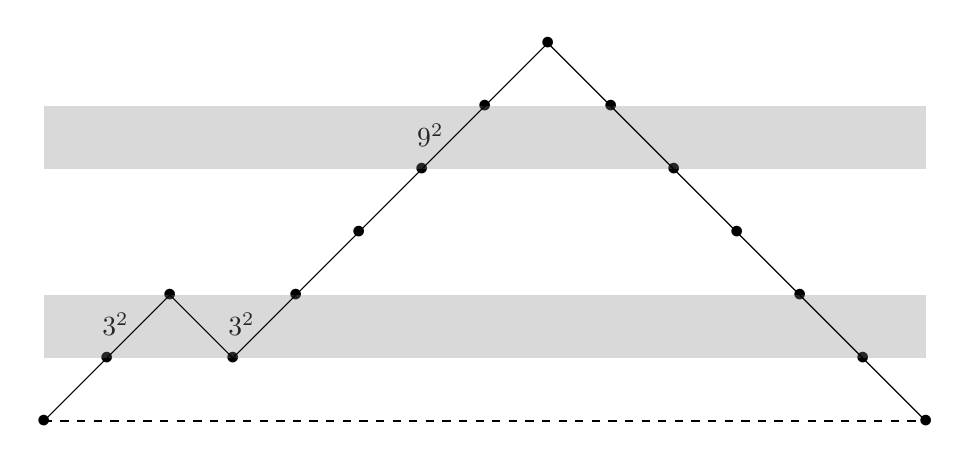
\begin{tikzpicture}[scale=0.8]
    \node at (0,0) {$\bullet$};
    \node at (1,1) {$\bullet$};
    \node at (2,2) {$\bullet$};
    \node at (3,1) {$\bullet$};
    \node at (4,2) {$\bullet$};
    \node at (5,3) {$\bullet$};
    \node at (6,4) {$\bullet$};
    \node at (7,5) {$\bullet$};
    \node at (8,6) {$\bullet$};
    \node at (9,5) {$\bullet$};
    \node at (10,4) {$\bullet$};
    \node at (11,3) {$\bullet$};
    \node at (12,2) {$\bullet$};
    \node at (13,1) {$\bullet$};
    \node at (14,0) {$\bullet$};
    \node[above left] at (1.5, 1.2) {$3^2$};
    \node[above left] at (3.5, 1.2) {$3^2$};
    \node[above left] at (6.5, 4.2) {$9^2$};
    \fill[fill=gray, fill opacity = 0.3] (0, 1)--(14, 1)--(14, 2)--(0, 2)--cycle;
    \fill[fill=gray, fill opacity = 0.3] (0, 4)--(14, 4)--(14, 5)--(0, 5)--cycle;
    \draw(0,0)--(2,2)--(3,1)--(8,6)--(14,0);
    \draw[dashed](0,0)--(14,0);
    \end{tikzpicture}
    
    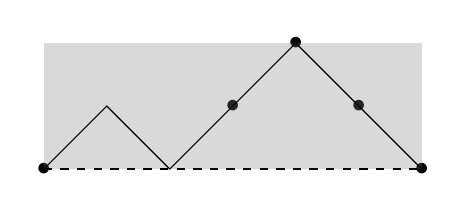
\begin{tikzpicture}[scale=0.8]
    \node at (0,0) {$\bullet$};
    \node at (3,1) {$\bullet$};
    \node at (4,2) {$\bullet$};
    \node at (5,1) {$\bullet$};
    \node at (6,0) {$\bullet$};
    \fill[fill=gray, fill opacity = 0.3] (0, 0)--(6, 0)--(6, 2)--(0, 2)--cycle;
    \draw(0,0)--(1, 1)--(2,0)--(4,2)--(6,0);
    \node[white] at (1,1) {};
    \node[white] at (2,0) {};
    \draw[dashed](0,0)--(6,0);
    \end{tikzpicture}
    \caption{A Dyck path for $n=7$, and its $3$-power path. The white vertices are marked because $P$ stays within the gray region.}
    \label{fig:powerpath}
    \end{figure}
    
    See Figure \ref{fig:powerpath} for an example. Visually, we shade in all levels for which the weight is a multiple of three and reduce only to steps which fall within the shaded regions. The marked vertices (white vertices) indicate when the path stayed in a shaded region for two consecutive steps.
    
    If $\alpha(P)$ has semilength $k$, then the weight of $P$ is divisible by $3^{2k}$ because each upward edge of $\alpha(P)$ corresponds to an upward edge of $P$ with weight divisible by $3^2$. We may write
    \[L_n=\sum_{P}\wt(P)=\sum_{\beta}\sum_{P: \alpha(P)=\beta}\wt(P)\]
    where the first sum is over all Dyck paths $P$ of semilength $n$, the second sum is over all $3$-power paths $\beta$, and the third sum is over all $P$ of semilength $n$ such that $\alpha(P)=\beta$. Modulo $3^r$, we only need to consider $\beta$ of semilength at most $\left\lfloor\frac{r-1}{2}\right\rfloor$ because otherwise $\wt(P)$ is divisible by $3^r$.
    
    Next we develop a formula for $\sum_{P: \alpha(P)=\beta}\wt(P)$ when $\beta$ is fixed. Let $\beta$ have semilength $k$. Consider a vertex $v$ of $\beta$ and let $e_L$ and $e_R$ be the edges to the left and right. These two edges correspond to some edges $e_L'$ and $e_R'$ of the original path $P$. Let $G(v)$ be the edges between $e_L'$ and $e_R'$. (If $v$ is the first or last vertex of $\beta$, then $G(v)$ consists of the first or last segment of $P$ that does not touch a gray region.)
    
    Note that by definition, $G(v)$ is empty whenever $v$ is a marked vertex. Furthermore, $G(v)$ is always nonempty whenever $v$ is not marked, because if $e_1$ and $e_2$ are in the same direction then $e_L'$ and $e_R'$ cannot be adjacent in $P$ because they are at different levels, and if they are not in the same direction then $e_L'$ and $e_R'$ cannot be adjacent in $P$ because $v$ was not marked.
    
    Enumerating the vertices of $\beta$ as $v_0, v_1, \dotsc, v_{2k}$ and the edges as $e_1, e_2, \dotsc, e_{2k}$ the path $P$ may be written as the union \[P=G(v_0)\cup e_1 \cup G(v_1)\cup \dotsb \cup e_{2k}\cup G(v_{2k}).\]
    We have already observed that from $\beta$ alone, we can determine if $G(v)$ is empty or not. Let $V_{0}$ be the set of vertices for which $G(v)$ is empty, and $V_1$ be the set of vertices for which $G(v)$ is nonempty. Furthermore, the parity of $\lvert G(v)\rvert$ is also always determined: it is even except when $v$ is the first or last vertex because the start and endpoints of $G(v)$ are at the same height or distance $2$.
    
    To create all paths $P$ with $\alpha(P)=\beta$, we will choose the tuple $(\lvert G(v_0)\rvert, \dotsc, \lvert G(v_{2k}\rvert)$ first, and then for each $v$ determine what the edges of $G(v)$ are conditioned on $\lvert G(v)\rvert$. We know some elements of $(\lvert G(v_0)\rvert, \dotsc, \lvert G(v_{2k}\rvert)$ are zero, while the rest are $1+2m$ or $2+2m$ where $m$ can be any nonnegative integer. The weight of $P$ can be written as the product of the weights of $G(v_i)$ and the edges $e_i$ associated with $\beta$.
    
    Consider a vertex $v\in V_1$. First consider the case where $v$ is a start or end vertex and $G(v)$ has $1+2m$ edges. Clearly there is only one possibility for $G(v)$, which is to alternate between $y=0$ and $y=1$.
    
    Now suppose $v$ is not a start or end vertex and $G(v)$ has $2+2m$ edges. In the case where the edges $e_{L}, e_{R}$ to the left and right of $v$ go upward and downward respectively, $G(v)$ must go up from the top of a gray strip, at the line $y=3j+2$ for some $k$. The first edge of $G(v)$ must go from $y=3j+2$ to $y=3j+3$, while the last edge of $G(v)$ must go from $y=3j+3$ to $y=3j+2$. The $2m$ edges in between can be partitioned into pairs: the second and third edge either follow the path $3j+3\to 3j+2\to 3j+3$ or $3j+3\to 3j+4\to 3j+3$, the same is true for the fourth and fifth edges, etc. There are $2^m$ possibilities for $G(v)$, and the sum of the weights of $G(v)$ over all possibilities is given by $b(3j+2)^2(b(3j+2)+b(3j+3))^m$.
    
    Likewise, if $e_{L}$ and $e_{R}$ are downward and upward respectively, the sum of the weights of $G(v)$ over all possibilities is given by $b(3j+3)^2(b(3j+2)+b(3j+3))^m$ for some $j$. (There is the exception where $v$ is at $y=0$ in $\beta$, which will be similar to the case where $v$ is at the ends and the total weight will be $1$.) If $e_{L}$ and $e_{R}$ are in opposite directions, then the sum of the weights of $G(v)$ over all possibilities is given by $b(3j+2)b(3j+3)(b(3j+2)+b(3j+3))^m$ for some $j$.
    
    These results can be summarized as follows: for each $v\in V_1$, we may assign a nonnegative integer $m_v$ so that $G(v)$ has $1+2m_v$ or $2+2m_v$ edges depending on whether $v$ is at the ends. The total number of edges is $2k+2\lvert V_1\rvert-2 +2\sum_{v\in V_1} m_v=2n$ so we have the constraint $\sum m_v = n-k-\lvert V_1\rvert+1$. For each $v\in V_1$, we may independently determine $G(v)$, and the sum of the weights across the possible $G(v)$ is of the form $d_va_v^{m_v}$ for some constants $d_v, a_v$. A key property here is that $a_v$ is never a multiple of $3$, because it is either $1$ or $b(3j+2)+b(3j+3)\equiv 2\pmod{3}$. (Recall that our weight function is $b(x)=(2x+1)^2$.)   
    
    %Is 3 not dividing a_v actually needed?
    
    In summary, for a given path $3$-power path $\beta$, we have
    \[\sum_{P: \alpha(P)=\beta}\wt(P)=D_{\beta}\sum_{i_1+\dotsb+i_{\ell}=n-c_{\beta}}a_1^{i_1}\dotsm a_{\ell}^{i_\ell}\]
    where 
    \begin{align*}
        \ell &= \lvert V_1\rvert \\
        c_{\beta} &=k+\lvert V_1\rvert-1 \\
        D_{\beta} &= \prod_{e\in \beta}\wt(e)\prod_{v\in V_1}d_v
    \end{align*}
    are some constants depending only on $\beta$, and the $a_i$ are constants depending only on $\beta$ which are also not multiples of $3$.
    Denote 
    \[f(n)=\sum_{i_1+\dotsb+i_{\ell}=n-c_{\beta}}a_1^{i_1}\dotsm a_{\ell}^{i_\ell}.\]
    We have the generating function
    \[\sum_{n\geq 0}f(n)x^n=\sum_{n\geq 0}\sum_{i_1+\dotsb+i_{\ell}=n-c_{\beta}}a_1^{i_1}\dotsm a_{\ell}^{i_\ell}x^n=\frac{x^{c_{\beta}}}{(1-a_1x)\dotsm (1-a_{\ell}x)}.\]
    Modulo $3$, this takes the form $\frac{x^{c_\beta}}{(1-x)^{a}(1+x)^b}$ for some $a, b$ with $a+b=\ell$. It is known that this implies with this generating function may be written as
    \[f(n)\equiv \sum_{i=0}^{a-1}\binom{n}{i}+\sum_{i=0}^{b-1}\binom{n}{i}(-1)^n\]
    for $n\geq c_{\beta}$ (see \cite{pinch1995recurrent}). By Lemma \ref{lem:binomperiod}, the period of the above sequence modulo $3$ is a divisor of $2\cdot 3^m$ where $3^m$ is the least power of $3$ which is greater than $\max(a, b)$.
    
    For now we will assume that $\beta$ goes above the line $y=1$. This implies several things: first $\ell\geq 4$ because at least four vertices are in $V_1$: the start and end, and the two vertices where the path must cross the line $y=1$. It also implies that $D_{\beta}$ is a multiple of $3^{2k+2}$ because one of the edges has weight $9^2$.
    
    Note that $\ell\leq 2k+1$. Then we can say that $m\leq \ell-1\leq 2k$ as $3^{\ell-1} > \ell \geq \max(a, b)$ for $\ell\geq 4$. The period of the sequence modulo $3$ will divide $2\cdot 3^{2k}$. We also have the initial conditions $f(c_{\beta})=1$ and $f(n)=0$ for all $n < c_{\beta}$. By Lemma \ref{lem:primepowerperiod}, the period of $f(n)\pmod{3^{r-2k-2}}$ is a divisor of $2\cdot 3^{r-3}$. As $D_{\beta}$ is divisible by $3^{2k+2}$, the period of $\sum_{P: \alpha(P)=\beta}\wt(P)\pmod{3^{r}}$ is a divisor of $2\cdot 3^{r-3}$.
    
    Now we consider cases where $\beta$ does not go above $y=1$. Such paths must zigzag between $y=0$ and $y=1$. We also assume that $\beta$ is not the empty path, as that path has $\sum_{\beta}\sum_{P: \alpha(P)=\beta}\wt(P)=1$ which is periodic. The generating function takes the form
    \[\frac{x^{c_\beta}}{(1-x)^a(1-74x)^b}\]
    for some $a, b$ (here $74=5^2+7^2$). We also have the condition $a\geq 2$, because the start and end vertices of $\beta$ always have $a_v=1$. Let $3^m$ be the least power of $3$ greater than $\max(a, b)-1$. Then the period of this sequence modulo $3$ is divides $2\cdot 3^{m}$. If $m\leq \ell-3=a+b-3$, then the period of $f(n)\pmod{3^{r-2k}}$ divides $2\cdot 3^{r-3}$ which will be enough. We can directly check that this rules out all cases with $\max(a, b)\geq 5$, and further verification of the finitely many remaining cases leaves the following pairs:
    \[(a, b) = (2, 0), (3, 0), (4, 0),  (2, 1).\]
    In the case $(a, b)=(4, 0)$, the period of $f(n)\pmod{3^{r-2k}}$ divides $3^{r-2k+1}$. Therefore we only need to consider when the semilength $k$ is at most $1$. In fact, there is no path with $(a, b)=(4, 0)$ and semilength at most $1$, so we can eliminate this case.
    
    In the other three cases, the period of $f(n)\pmod{3^{r-2k}}$ divides $2\cdot 3^{r-2k}$ and again it suffices to only consider $k\leq 1$. This leaves the following two paths $\beta_1, \beta_2$:
    \begin{center}
    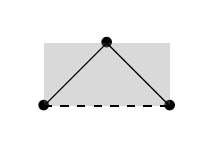
\begin{tikzpicture}[scale=0.8]
    \node at (0,0) {$\bullet$};
    \node at (1,1) {$\bullet$};
    \node at (2,0) {$\bullet$};
    \fill[fill=gray, fill opacity = 0.3] (0, 0)--(2, 0)--(2, 1)--(0, 1)--cycle;
    \draw(0,0)--(1, 1)--(2,0);
    \draw[dashed](0,0)--(2,0);
    \end{tikzpicture}
    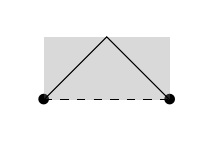
\begin{tikzpicture}[scale=0.8]
    \node at (0,0) {$\bullet$};
    \node at (2,0) {$\bullet$};
    \fill[fill=gray, fill opacity = 0.3] (0, 0)--(2, 0)--(2, 1)--(0, 1)--cycle;
    \draw(0,0)--(1, 1)--(2,0);
    \draw[dashed](0,0)--(2,0);
    \node[white] at (1,1) {};
    \end{tikzpicture}
    \end{center}
    We will group these paths together. With all the factors included, we have
    \begin{align*}
        \sum_{P: \alpha(P)=\beta_1}\wt(P) &= 9\cdot 25\cdot\sum_{i_1+i_2+i_3=n-3}74^{i_2} = 9\cdot 25\cdot \sum_{k=0}^{n-3}(n-2-k)74^k \\
        &=9\cdot 25\cdot\left(\frac{74^{n-1}}{73^2}-\frac{n}{73}+\frac{72}{73^2}\right). \\
        \sum_{P: \alpha(P)=\beta_2}\wt(P) &= 9(n-1). \\
    \end{align*}
    The sum of these two is
    \[g(n)=9\left(\frac{25}{73^2}\cdot 74^{n-1}+\frac{48}{73}n-\frac{3529}{73^2}\right).\]
    We claim that $T=2\cdot 3^{r-3}$ is a period of this function of $n$ modulo $3^r$. It suffices to show that $2\cdot 3^{r-3}$ is a period of $\frac{25}{73^2}\cdot 74^{n-1}+\frac{48}{73}n-\frac{3529}{73^2}\pmod{3^{r-2}}$. However, this is easy because $74^n$ has period $2\cdot 3^{r-3}$ (since $\varphi(3^{r-2})=2\cdot 3^{r-3}$) and $\frac{48}{73}n$ has period $3^{r-3}$ because $48$ is divisible by $3$.
    
    We finish the argument as follows: any $\beta$ with semilength greater than $\left\lfloor\frac{r-1}{2}\right\rfloor$ may be ignored, so we only have finitely many $\beta$ to consider in the summation
    \[L_n=\sum_{\beta}\sum_{P: \alpha(P)=\beta}\wt(P).\]
    For each $\beta$, the sum $\sum_{P: \alpha(P)=\beta}\wt(P)$ is eventually periodic in $n$ with period dividing $2\cdot 3^{r-3}$ (aside from the two paths which we grouped together). As there are finitely many $\beta$, we conclude that $L_n\pmod{3^r}$ is eventually periodic with period dividing $2\cdot 3^{r-3}$.
\end{proof}

\subsection{Further Morse link number conjectures}\label{subsec:valuationconjectures}

Postnikov also stated some conjectures regarding $2$ and $5$-adic valuations of sequences related to $L_n$. We rephrase some below and provide some further conjectures.

\begin{conjecture}[\cite{postnikov2000morse}]
    There exists a $2$-adic integer $\alpha=\dotsc 010111_2$ such that
    \[\xi_2(L_n-C_n)=s_2(n)+\xi_2(n-\alpha)+2\]
    for all $n\geq 2$.
\end{conjecture}

We generalize this conjecture as follows:

\begin{conjecture}
    Let $k$ be a positive integer and $L^{(k)}_n$ denote the weighted Catalan numbers with weight $b(x)=(2x+1)^{2k}$. There exists a $2$-adic integer $\alpha_k$ and nonnegative integer $c_k$ such that
    \[\xi_2(L_n^{(k)}-C_n)=s_2(n)+\xi_2(n-\alpha_k)+c_k\]
    for all $n\geq 2$.
\end{conjecture}

Similar phenomena were \emph{not} observed for other polynomial weight functions $b$ which satisfy the conditions of Theorem \ref{thm:postsagan}, suggesting that there is something special here.

\begin{conjecture}[\cite{postnikov2000morse}]
\label{conj:Morse5adic}
    If $\alpha$ is the $5$-adic integer $\dotsc 111111120_5$, then for $n\geq 4$ we have
    \[\xi_5(L_n)=\begin{cases}
    2 &\text{ if $n$ is even} \\
    \xi_5(n-\alpha)+3 &\text{ if $n$ is odd}
    \end{cases}.\]
\end{conjecture}
Note that the original conjecture in \cite{postnikov2000morse} contains some typos.

From computational evidence, it appears that $\xi_3(L_n-1)$ also follows a type of pattern but it may not be as simple as the one given in Conjecture \ref{conj:Morse5adic}. We suggest the following:

\begin{conjecture}
\label{conj:Morse3adic}
    There exists a $3$-adic integer $\alpha$ such that for odd $n\geq 3$, the quantity $\xi_3(L_n-1)$ depends only on $\xi_3(n-\alpha)$ and the last digit of $\frac{n-\alpha}{3^{\xi_3(n-\alpha)}}$, which is $1$ or $2$.
\end{conjecture}
If Conjecture \ref{conj:Morse3adic} were true, then for $n\geq 3$ we would have
\[\xi_3(n) =\begin{cases}
2 & n\text{ even} \\
6 & n\equiv 1\pmod{6} \\
4 & n\equiv 3\pmod{6} \\
5 & n\equiv 5, 11 \pmod{18} \\
\vdots
\end{cases}.\]